%% Ankur Sinha

%% packages %%
% support for coloured text
\usepackage{xcolor}
% moreland colour palette:
% https://github.com/Gnuplotting/gnuplot-palettes/blob/master/moreland.pal
% create: blue
\definecolor{moreland1}{HTML}{3b4cc0}
%visualise
\definecolor{moreland2}{HTML}{688aef}
%validate
\definecolor{moreland3}{HTML}{99baff}
%simulate
\definecolor{moreland4}{HTML}{c9d8ef}
%fit
\definecolor{moreland5}{HTML}{edd1c2}
%share
\definecolor{moreland6}{HTML}{f7a789}
%reuse
\definecolor{moreland7}{HTML}{e36a53}
% extra: red
\definecolor{moreland8}{HTML}{b40426}

% set 1 colour palette
% https://github.com/Gnuplotting/gnuplot-palettes/blob/master/set1.pal
% red
\definecolor{set11}{HTML}{E41A1C}
% blue
\definecolor{set12}{HTML}{377EB8}
% green
\definecolor{set13}{HTML}{4DAF4A}
% purple
\definecolor{set14}{HTML}{984EA3}
% orange
\definecolor{set15}{HTML}{FF7F00}
% yellow
\definecolor{set16}{HTML}{FFFF33}
% brown
\definecolor{set17}{HTML}{A65628}
% pink
\definecolor{set18}{HTML}{F781BF}

% IPA
\usepackage{tipa}
\usepackage[scale=2]{ccicons}
\usepackage{amssymb}
\usepackage{standalone}
\usepackage{tikz}
\usetikzlibrary{shapes.geometric,arrows,positioning,quotes,graphs,mindmap,decorations.pathmorphing,trees}
\usepackage{jneurosci}
\usepackage{subcaption}
\usepackage[T1]{fontenc}
\usepackage[utf8]{inputenc}
\usepackage[style=nature,backend=biber,autocite=footnote]{biblatex}
\addbibresource{/home/asinha/Documents/01_Readables/00_research_papers/bibliography/masterbib.bib}
\usepackage{roboto}
% for strike through
\usepackage[normalem]{ulem}
% links, urls, refs
\usepackage{hyperref}
\hypersetup{colorlinks,linkcolor=Green,urlcolor=set18}
% graphics
\usepackage{graphicx}
\graphicspath{{99_images/}}
% algorithm
\usepackage{algorithmic}
\usepackage{textcomp}
\usepackage{wrapfig}
\usepackage{textgreek}
\usepackage{euler}
\usepackage{tabularx}
\usepackage{booktabs}
\usepackage{minted}
\usepackage{csquotes}
\usepackage{movie15}
% beamer theme
% use defaults for theme
\usetheme[progressbar=foot]{moloch}
% for page numbers
\setbeamertemplate{page number in head/foot}[appendixframenumber]
% for footnotes
% https://tex.stackexchange.com/questions/683533/beamer-theme-metropolis-does-not-allow-different-font-size-for-fullcite/683540#683540
\setbeamerfont{bibliography entry title}{size=}
\setbeamerfont{bibliography entry author}{size=}
\setbeamerfont{bibliography entry location}{size=}
\setbeamerfont{bibliography entry note}{size=}
%\usetheme[numbering=fraction,sectionpage=progressbar,subsectionpage=progressbar,progressbar=frametitle]{metropolis}
%\usefonttheme[onlymath]{serif}
\setbeamerfont{footnote}{size=\Tiny}
\setbeamerfont{caption}{size=\tiny}
\setbeamercolor{alerted text}{fg=Green}
\setbeamerfont{note page}{size=\small}
\setbeamercolor{alerted text}{fg=set15}
\setbeamercolor{progress bar}{fg=set18}
\setbeamercolor{title separator}{fg=set18}
\setbeamercolor{frametitle}{bg=moreland1}

\renewcommand{\figurename}{}

% Not needed in metropolis, but in general footnote citation fixes: https://tex.stackexchange.com/questions/44217/how-can-i-stop-footcite-from-hijacking-my-beamer-columns
% how to use multiple references to the same footnote: https://tex.stackexchange.com/questions/27763/beamer-multiple-references-to-the-same-footnote

% Disable footnoterule
\renewcommand{\footnoterule}{}
\renewcommand*{\bibfont}{\tiny}

%% title %%
\title{Computational modelling at the Silver Lab}
\subtitle{NeuroML, Open Source Brain, OpenWorm, MDF}
\author[Ankur Sinha]{Ankur Sinha\\Padraig Gleeson\\R Angus Silver\\https://silverlab.org}
\date{2024-10-21}

%% document begins %%
\begin{document}


% title frame %%
\begin{frame}
  \titlepage{}
\end{frame}
%% Three slides for 5 minutes seems good
%% So, 30 slides at most for 50 minutes

% Why is biophysically detailed modelling important?
% Why are standards necessary?
%\section{Biophysically detailed models and standards}
%\section{NeuroML}
\begin{frame}[c]
  \frametitle{NeuroML: data driven biophysically detailed modelling}
  \begin{figure}[h]
    \centering
    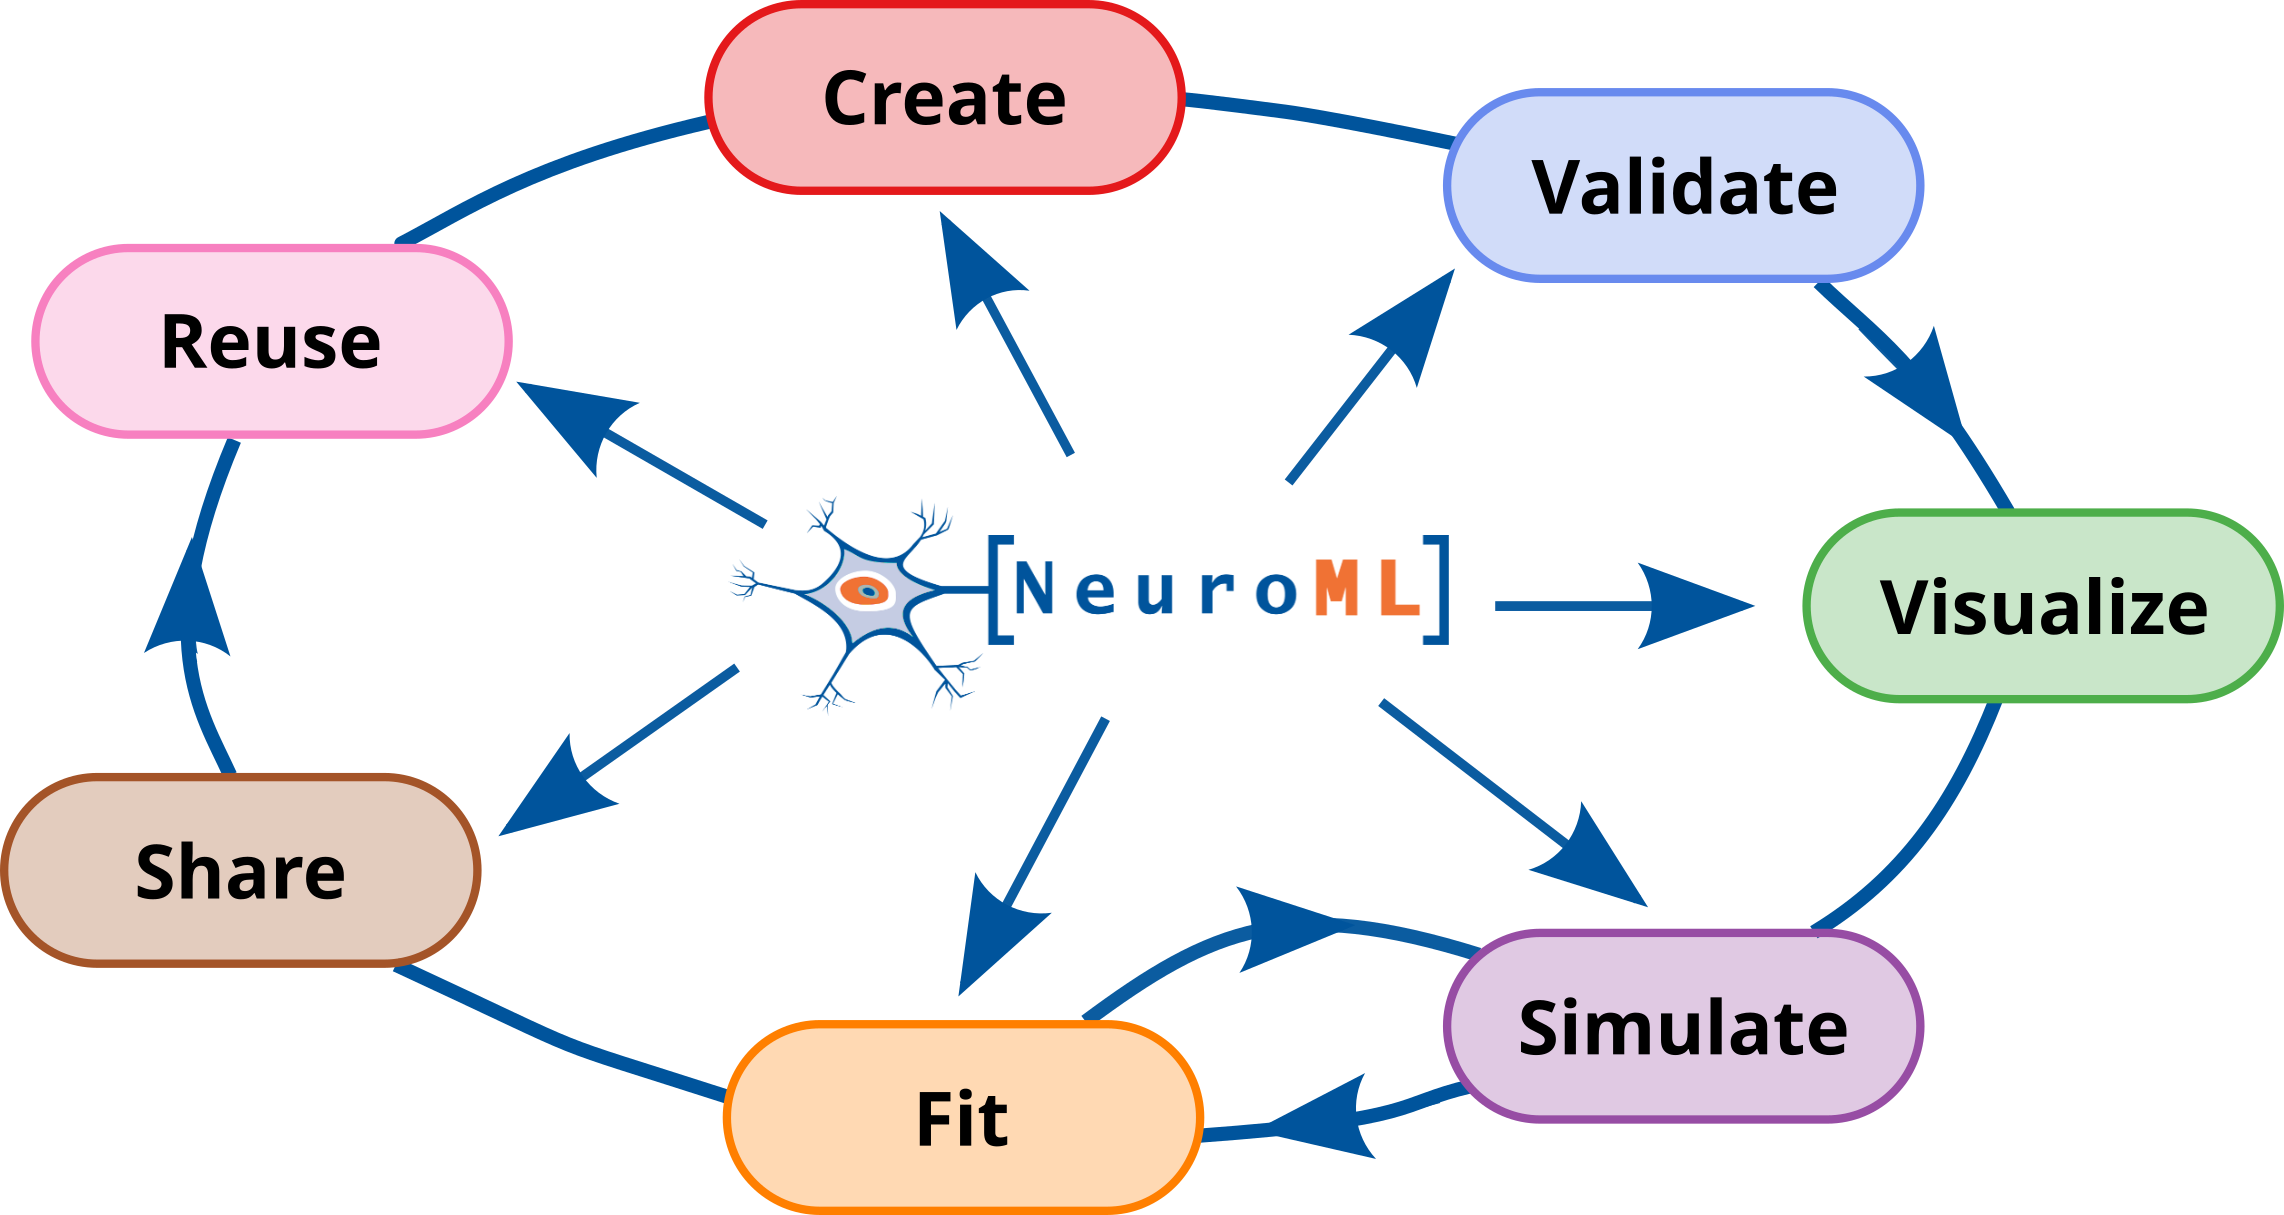
\includegraphics[width=\textwidth]{99_images/ecosystem}
  \end{figure}
\note[item]{The idea being that by being the standard, various tools that support various stages of the model life cycle can then work together.}
\end{frame}
\begin{frame}[c]
  \frametitle{NeuroML standard: curated model elements}
  \begin{figure}[h]
    \centering
    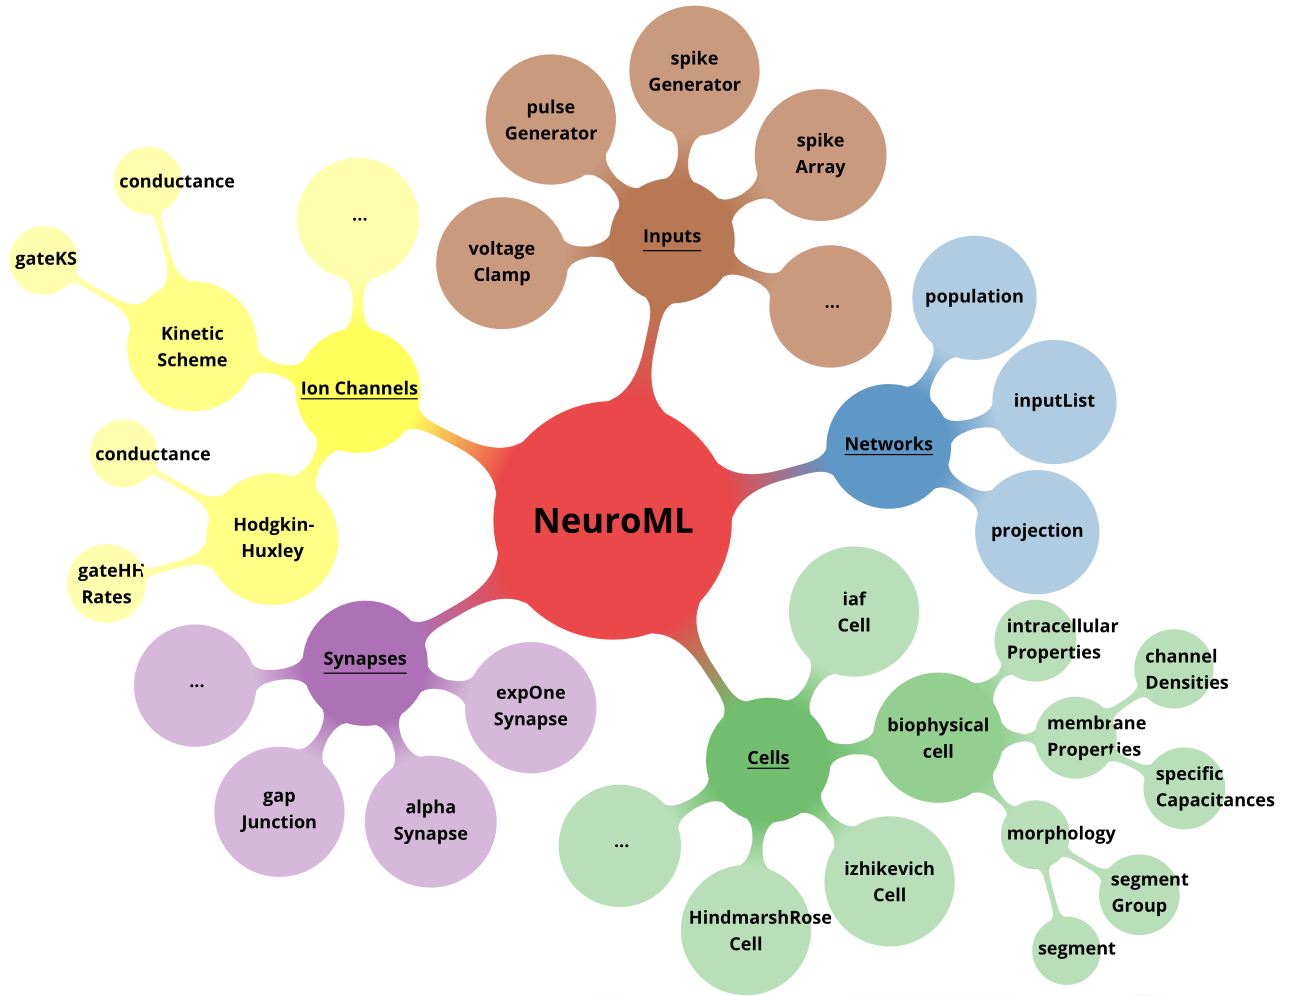
\includegraphics[width=0.9\textwidth]{99_images/neuroml-mindmap}
  \end{figure}%
  \footnotetext[1]{Full standard is at:~\url{https://docs.neuroml.org/Userdocs/Specification.html}}
\note[item]{An important aspect of the standard is that it includes lots of commonly used model elements already.}
\note[item]{So that users don't have to write these themselves, they can use the ones already provided.}
\note[item]{The mind map shows you a sub-set of model elements included in the NeuroML standard.}
\end{frame}
\begin{frame}[c]
  \frametitle{NeuroML software ecosystem}
  \begin{figure}[t]
    \begin{figure}[h]
      \centering
      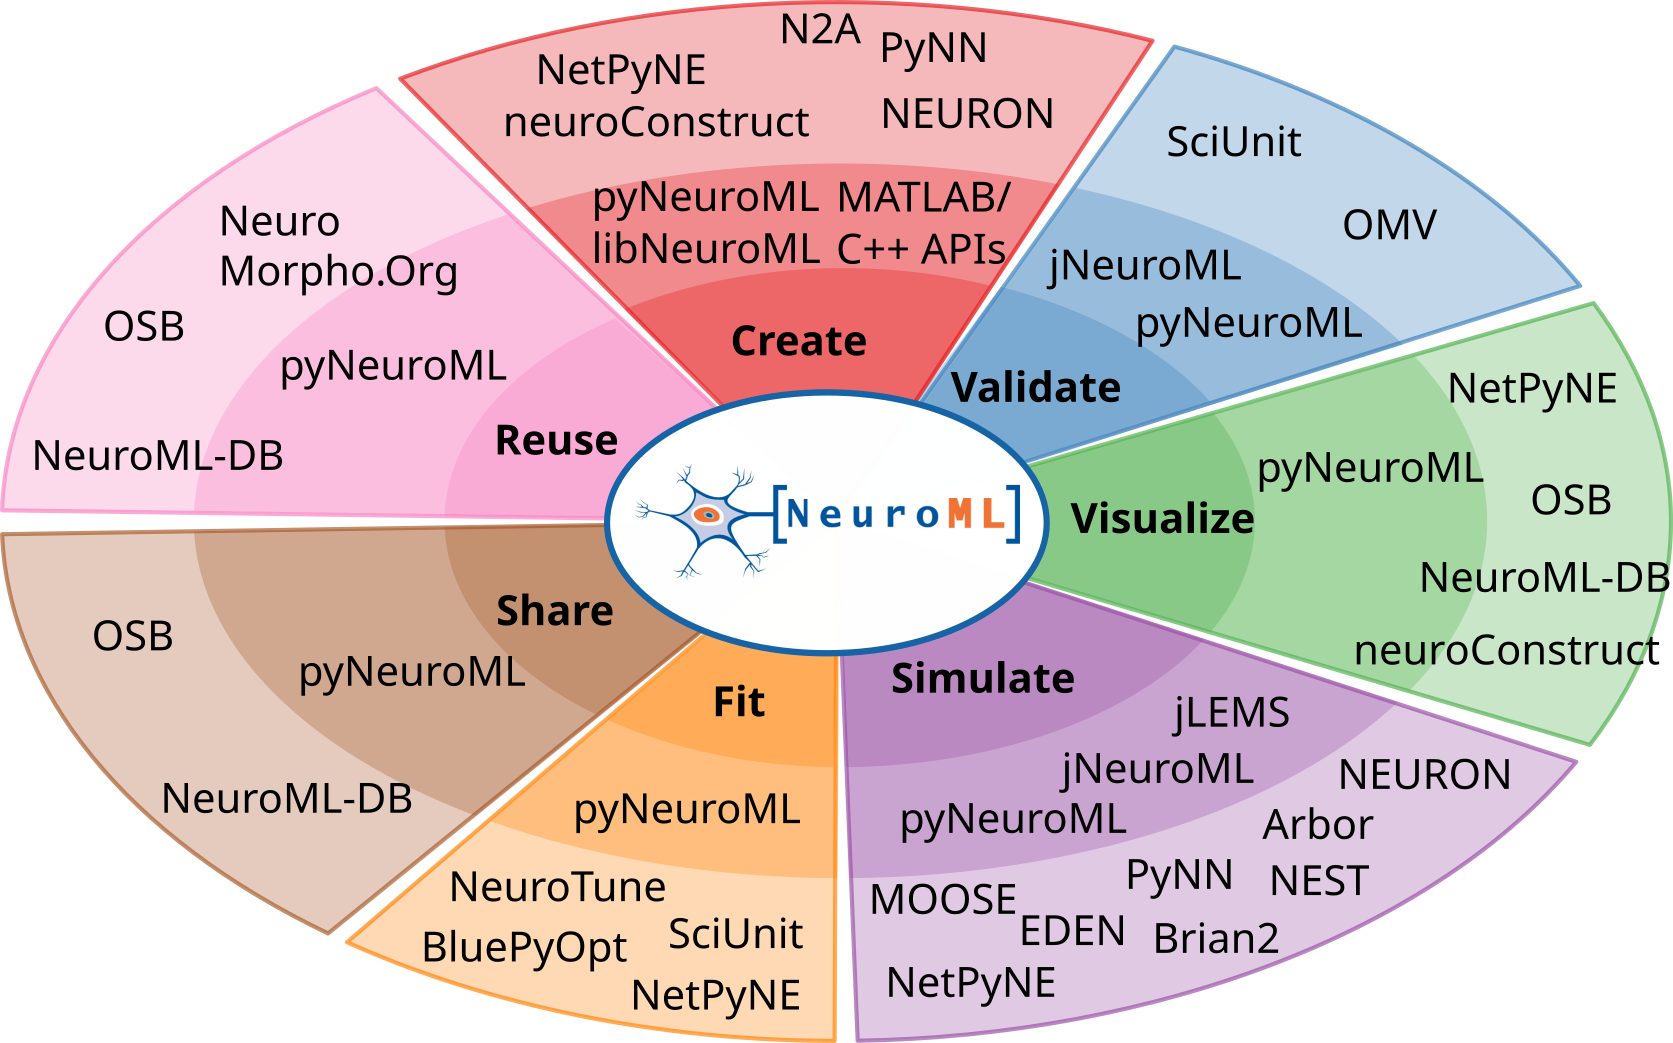
\includegraphics[width=0.9\textwidth]{99_images/ecosystem-onion}
    \end{figure}%
  \end{figure}
\note[item]{An important aspect of the standard is that it includes lots of commonly used model elements already.}
\note[item]{So that users don't have to write these themselves, they can use the ones already provided.}
\note[item]{The mind map shows you a sub-set of model elements included in the NeuroML standard.}
\end{frame}
\begin{frame}[c]
  \frametitle{NeuroML: linking with other standards}
  \begin{figure}[h]
    \centering
    
\includegraphics[width=0.7\textwidth]{99_images/neuroml-logo}\\\vspace{0.2cm}
  \end{figure}%
  \begin{columns}
    \begin{column}{0.5\textwidth}
      \begin{figure}[h]
        \centering
        
\includegraphics[width=0.7\textwidth]{99_images/sedml}\\\vspace{0.2cm}
      \end{figure}%
    \end{column}
    \begin{column}{0.5\textwidth}
      \begin{figure}[h]
        \centering
        
\includegraphics[width=0.7\textwidth]{99_images/sbml}
      \end{figure}%
    \end{column}
  \end{columns}
\end{frame}
\begin{frame}[c]
  \frametitle{NeuroML: publication}
  \begin{center}
    
\includegraphics[keepaspectratio,width=\textwidth]{./99_images/20241018-neuroml-elife}\\\vspace{1ex}
    \url{https://docs.neuroml.org}
  \end{center}
\end{frame}
\begin{frame}[c]
  \frametitle{Open Source Brain: scalable integrated research environment}
  \begin{center}
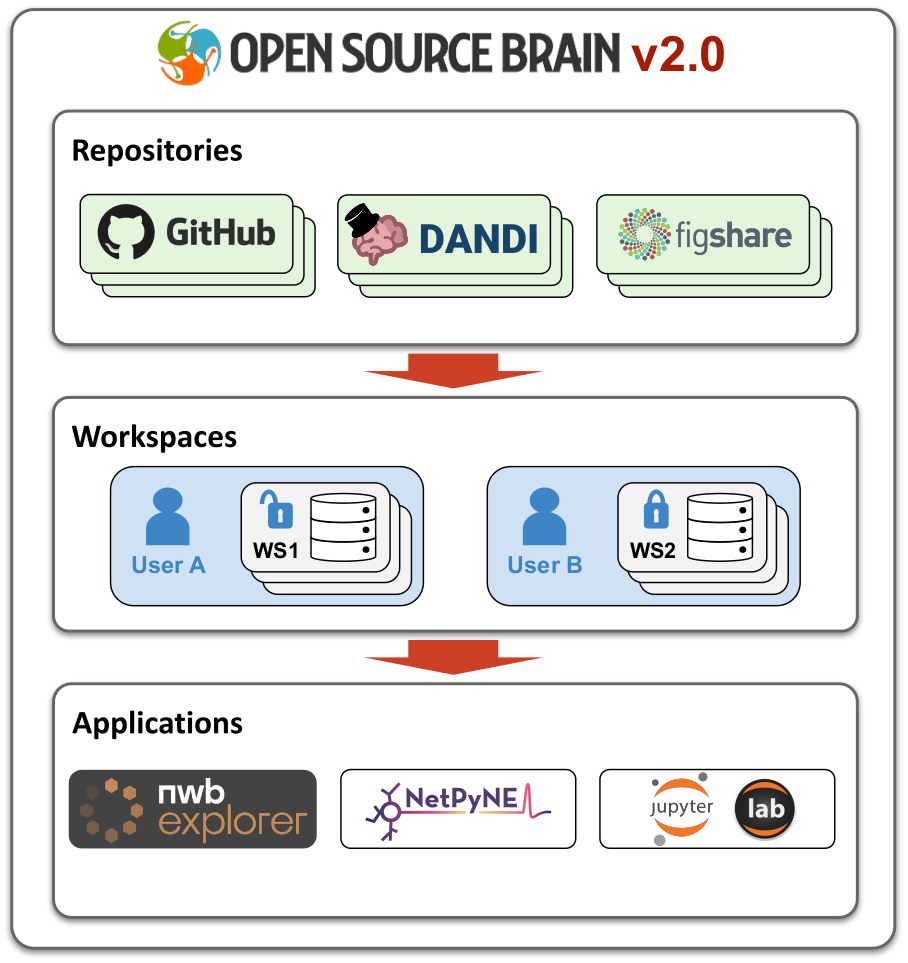
\includegraphics[keepaspectratio,height=0.9\textheight]{./99_images/OSBv2Overview}
  \end{center}
\end{frame}
\begin{frame}[c]
  \frametitle{Open Source Brain: applications}
  \begin{center}
    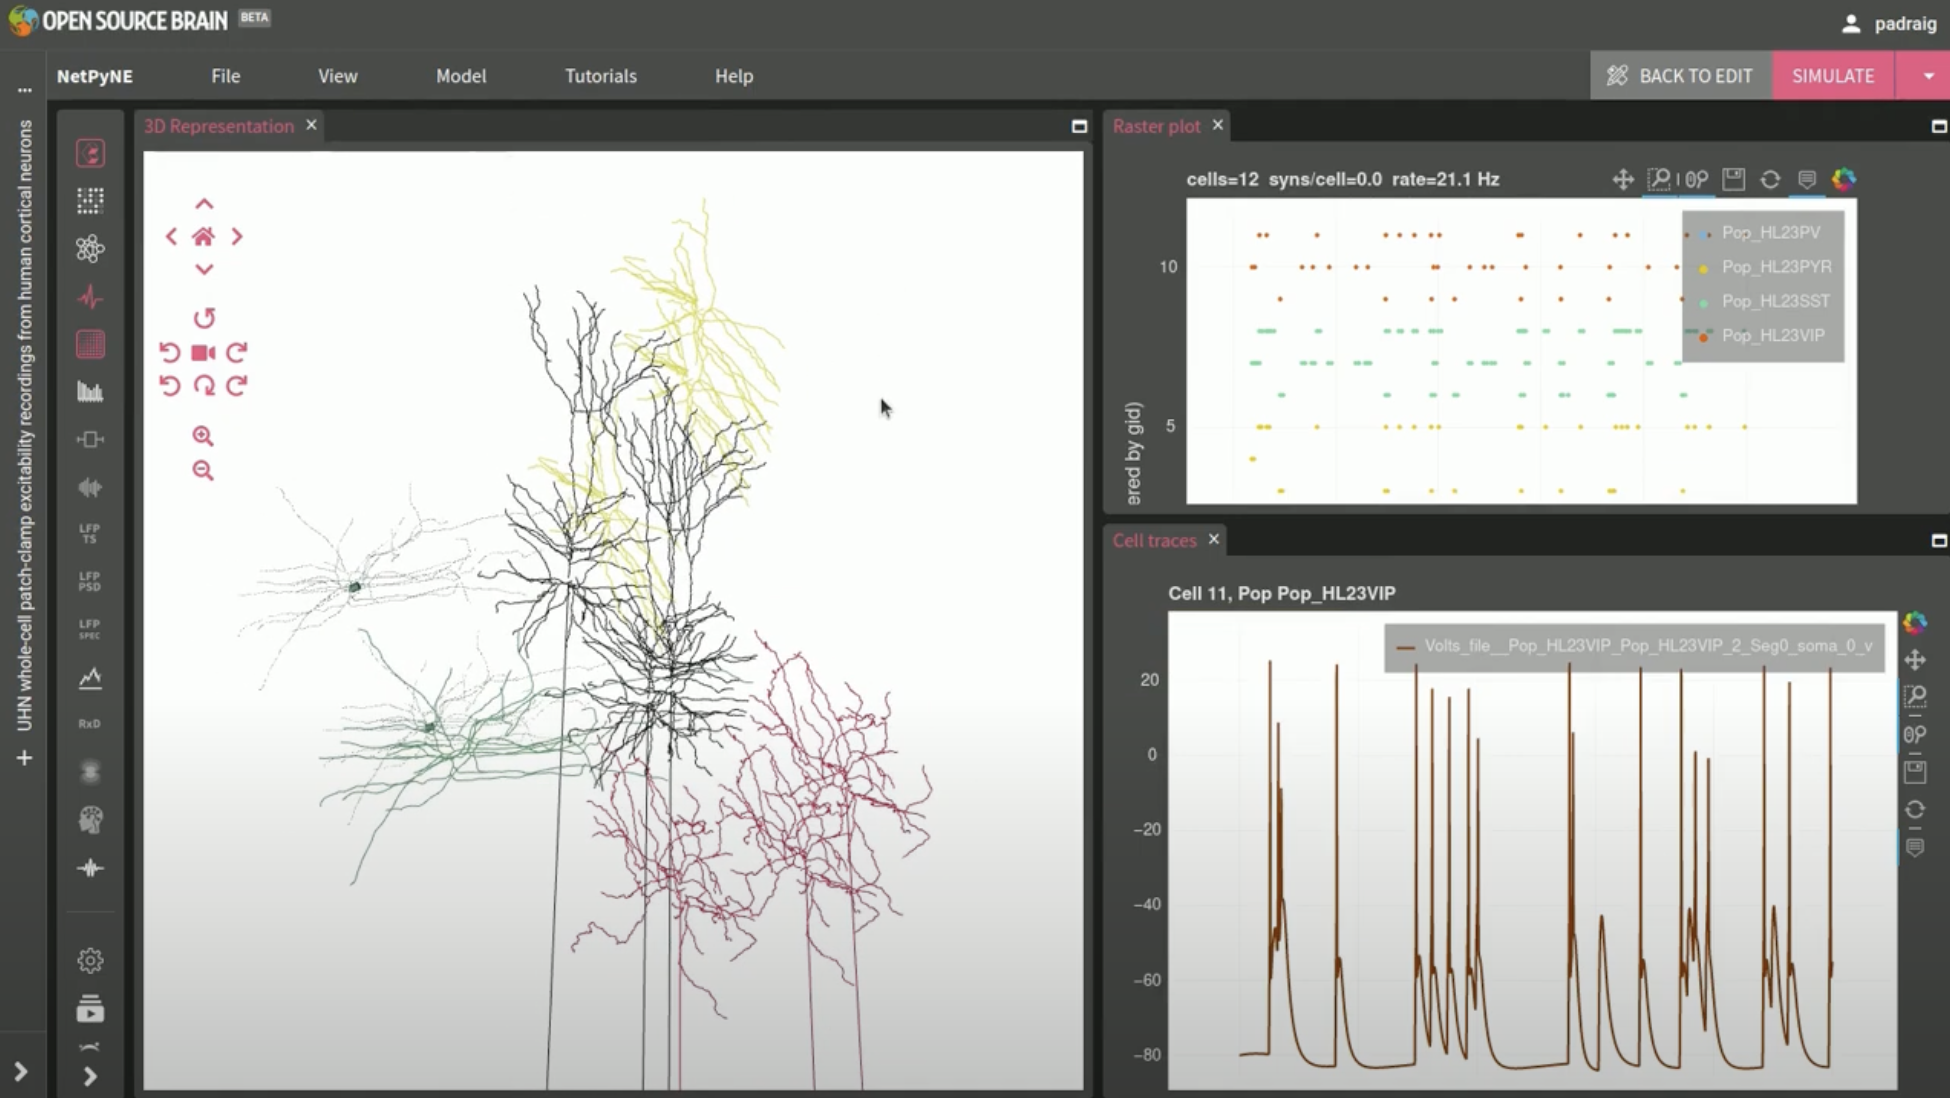
\includegraphics[keepaspectratio,width=0.49\textwidth]{./99_images/Netpyne}
    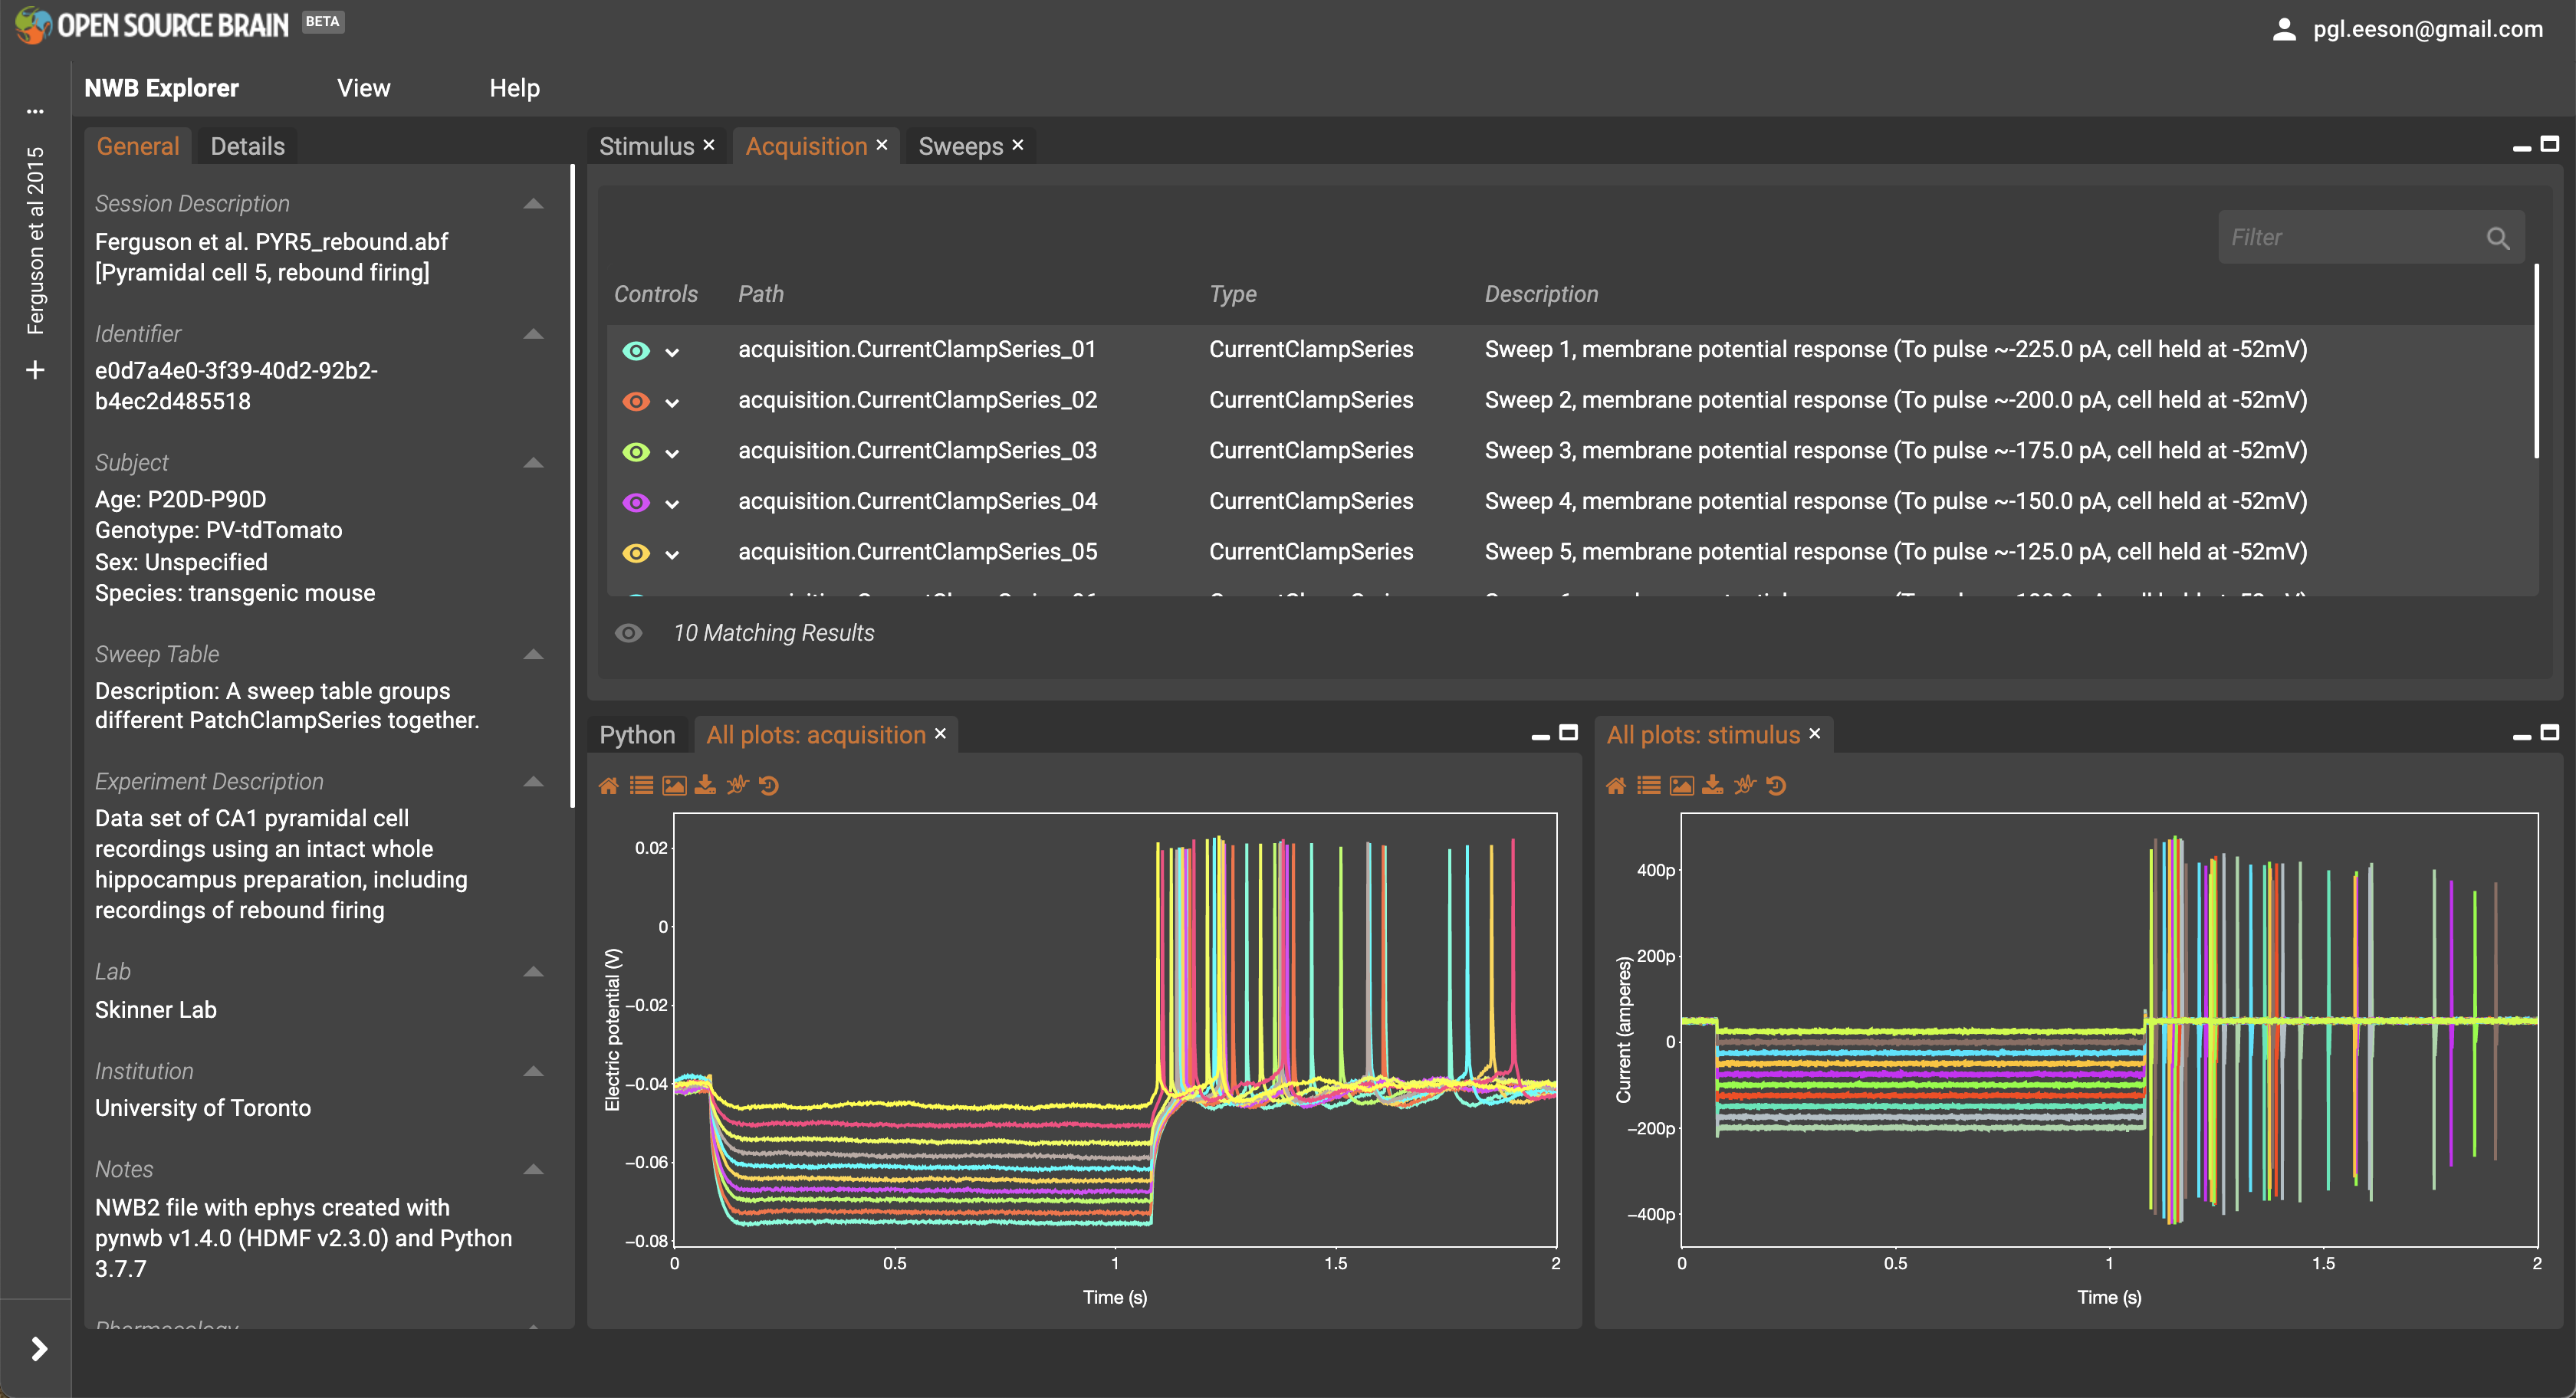
\includegraphics[keepaspectratio,width=0.5\textwidth]{./99_images/nwbe}\\\vspace{2ex}
    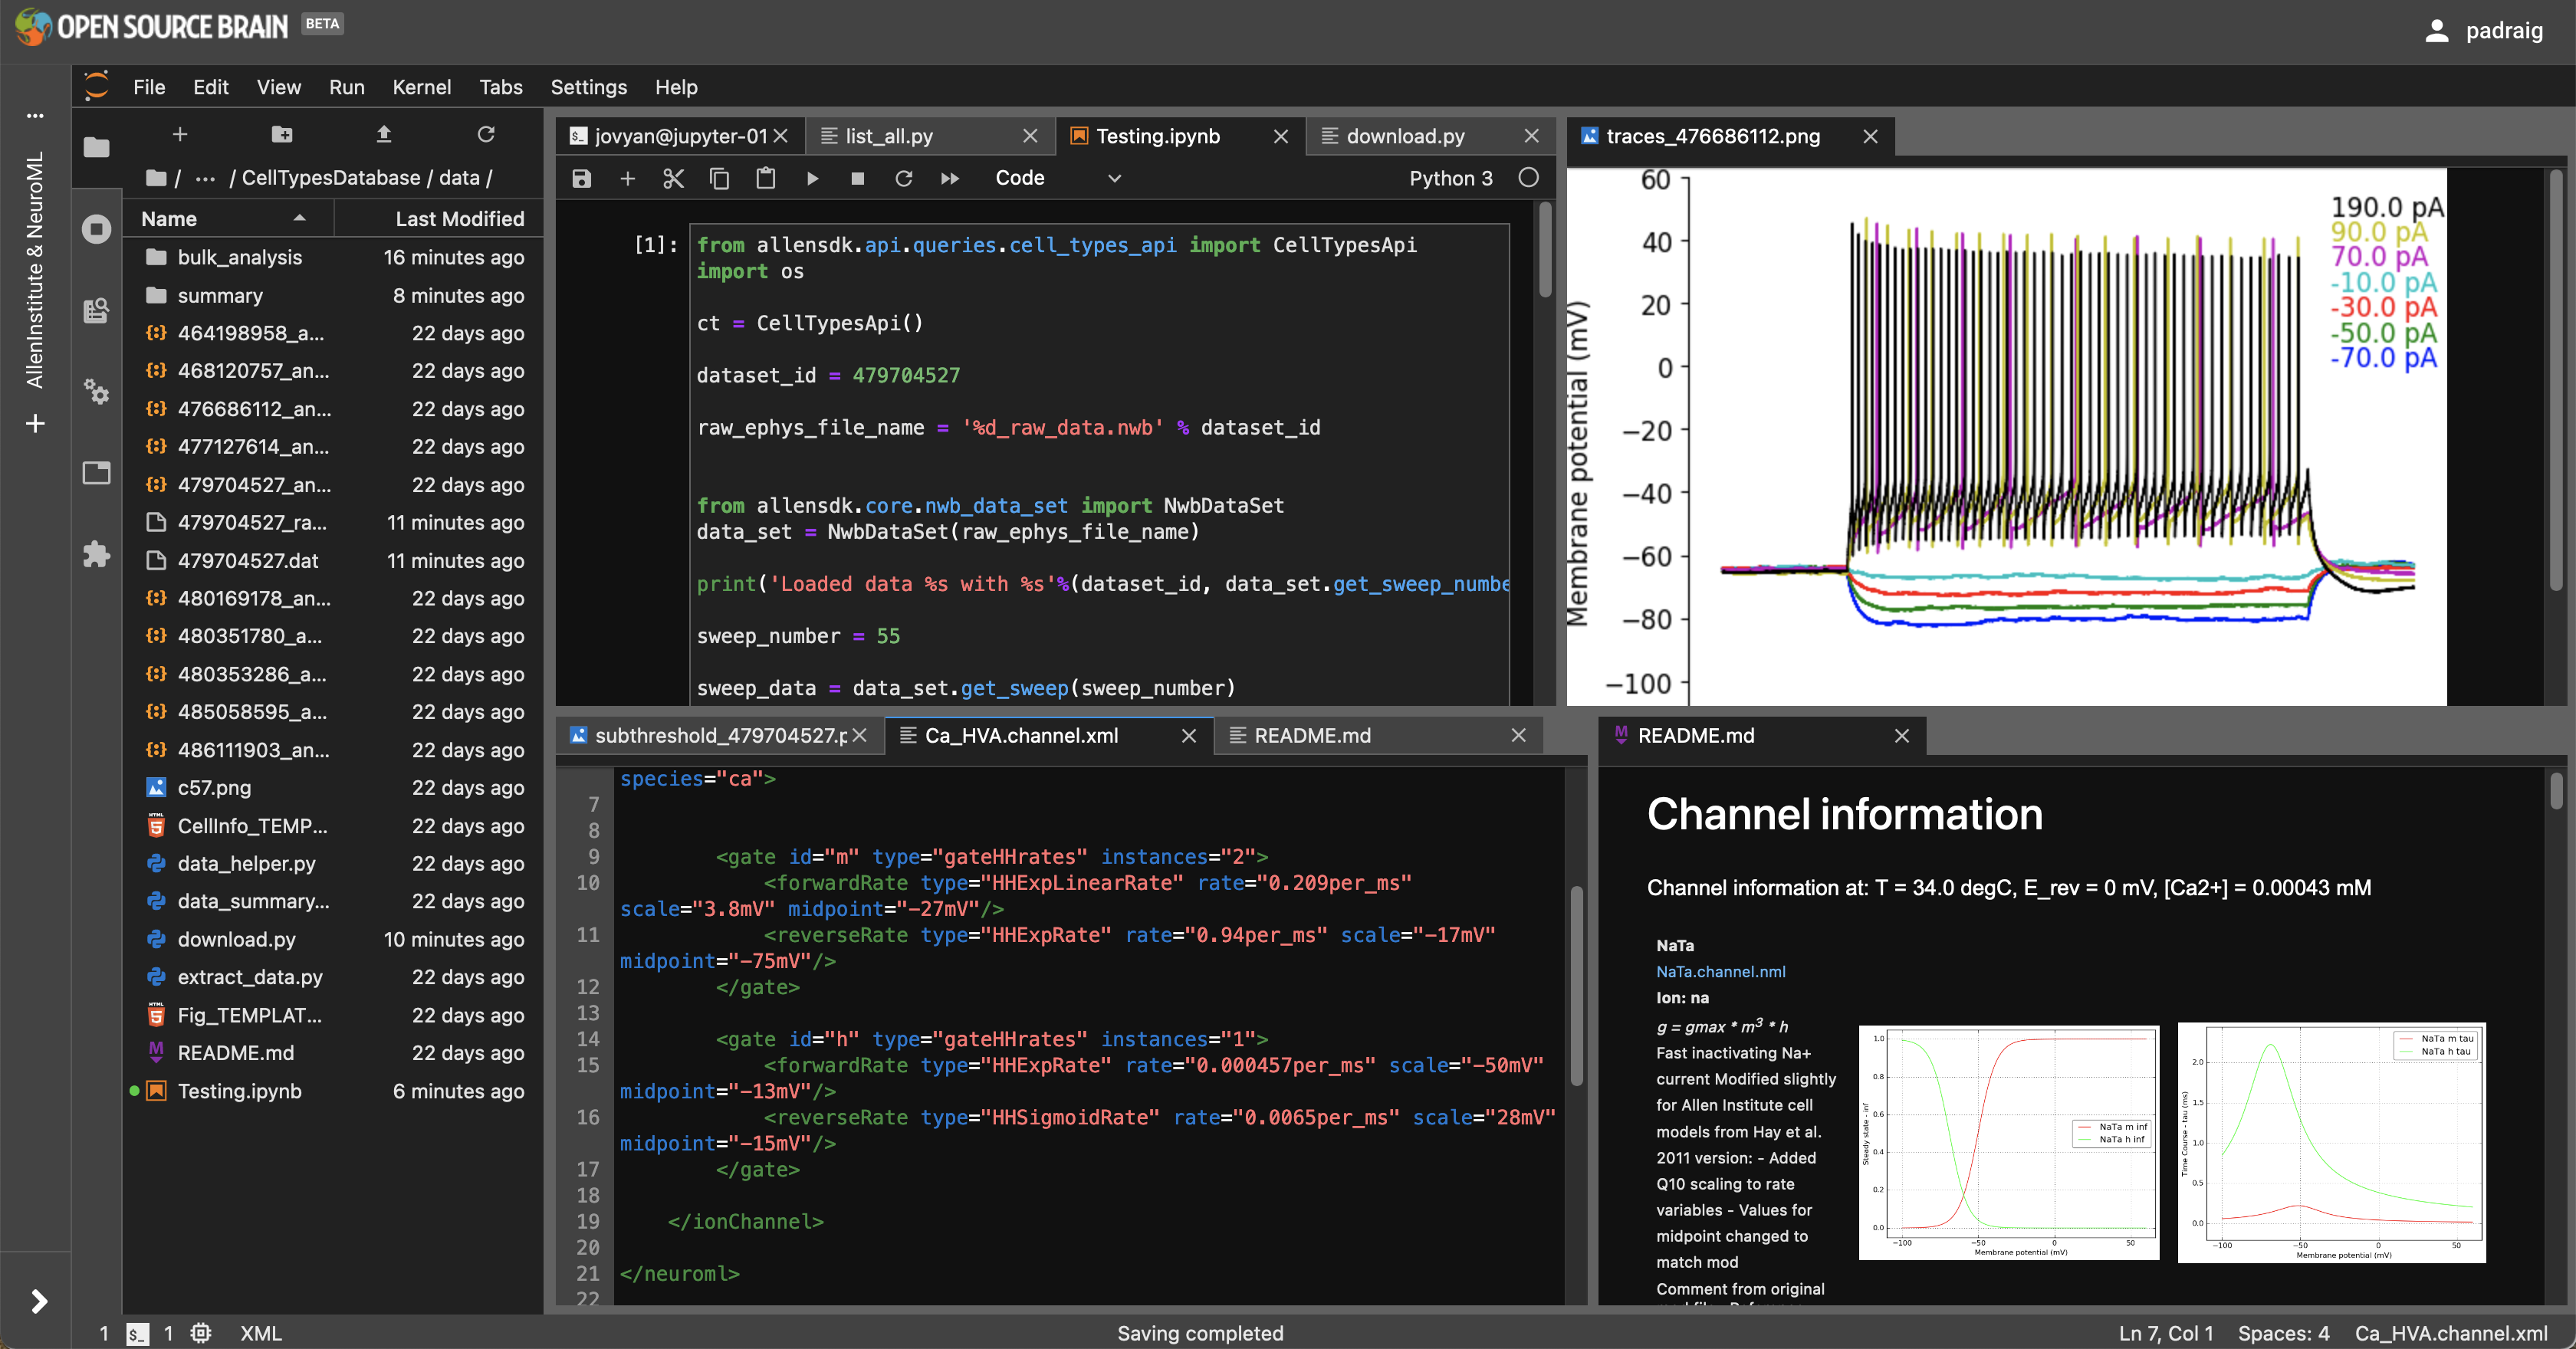
\includegraphics[keepaspectratio,width=0.5\textwidth]{./99_images/jlab}\\\vspace{1ex}
    \url{https://opensourcebrain.org}
  \end{center}
\end{frame}
\begin{frame}[c]
  \frametitle{Open Worm: open C elegans modelling and research}
  \begin{center}
    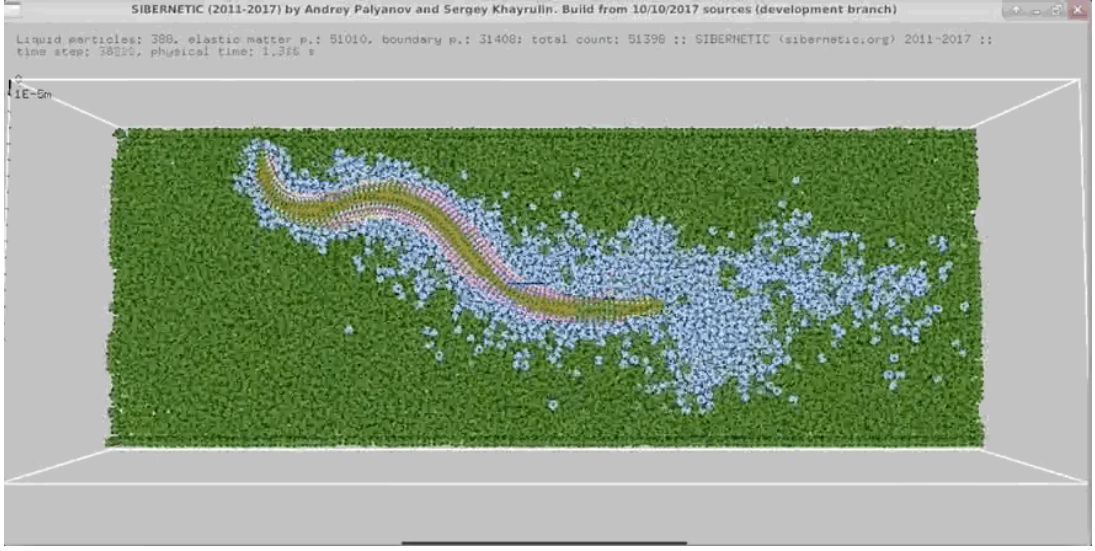
\includegraphics[keepaspectratio,width=\textwidth]{./99_images/sibernetic}\vspace{1ex}
    \url{https://openworm.org}
  \end{center}
\end{frame}
\begin{frame}[c]
  \frametitle{MDF: linking different types of modelling}
  \begin{center}
    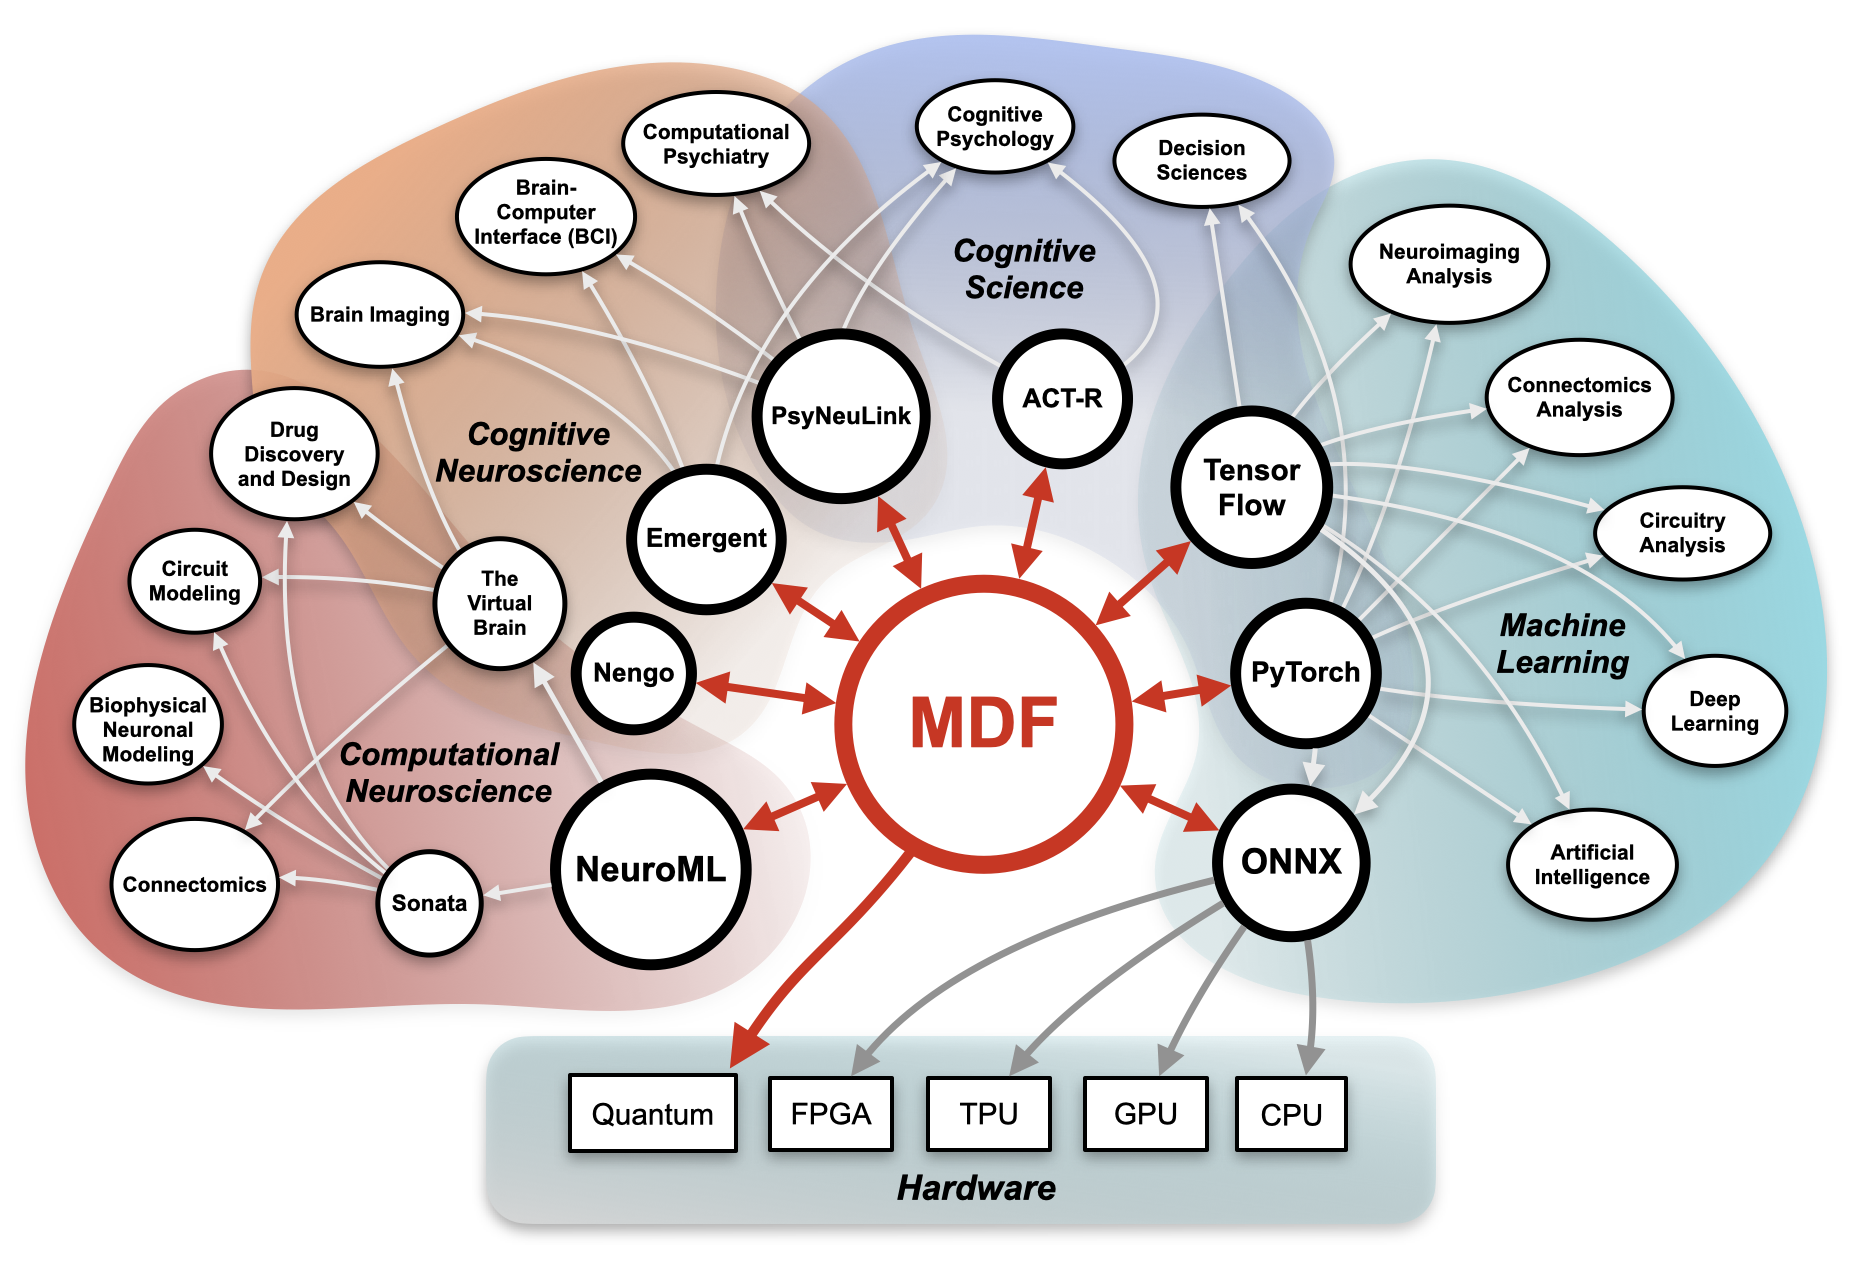
\includegraphics[keepaspectratio,width=\textwidth]{./99_images/mdf}\vspace{1ex}
    \url{https://modeci.org}
  \end{center}
\end{frame}
\end{document}
